\section{Area Comparisons}
This report shows how a robust address and pattern generation scheme can be implemented with very little increase in area.  The implementation does require some additional area over the base design.  For large memory blocks, the address generator only requires 0.6\% more area overhead than the base design.  Similarly, the pattern generator adds 1.0\% more area within the memory block.  For designs using an auxiliary memory, the pattern generator reduces the overall memory area by 50\%.  

\label{sect:cln-area}
\subsection{Address Geneator Area}
The original base design only offered binary and LFSR up/down counters for address counting methods.  The proposed design improves on the base design by providing a more robust address counting method that industry uses to test memory during production.  Table \ref{table:ac_area_compare} below shows the area increases by  59.3\% for the address counter block and 17.7\% for the overall PMBIST area.  

\begin{table}[ht]
\caption{Address Counter Area (\textit{um\textsuperscript{2}})}
\centering
\begin{tabular}{| l | l | l | l |}
\hline
Component & Base Design & Proposed Design & Percentage Difference \\ [0.5ex]
\hline\hline
address counter & 1810   & 2884   & 59.3\% \\
pmbist area     & 6057   & 7132   & 17.7\% \\ 
\hline
\end{tabular}
\label{table:ac_area_compare}
\end{table}

It is important to note the overall area diffence with respect to the full memory block.  This can be interpreted as the area cost for the additional address counting methods that ease manufacturing tests and add more robustness to the PMBIST.  Table \ref{table:ac_area_overhead} shows the percentage of the total memory block used by the original and proposed address counter designs.  As the memory sizes increase, the area increase due to the address generator becomes insignificant when the benefits of the new addressing schemes are considered.   

\begin{table}[ht]
\caption{Address Counter Area within Memory Block}
\centering
\begin{tabular}{p{0.5in} p{1.25in} | l | l | l |  }
\cline{3-5}
& & \multicolumn{3}{ c| }{Area Overhead Percentages} \\
\hline
\multicolumn{1}{|p{0.5in}|}{Memory Size} & Total Memory Area (\textit{um\textsuperscript{2}}) & Base Design & Proposed Design & Difference \\ [1ex]
\hline\hline
\multicolumn{1}{|c|}{64x8  }  & 15780  & 27.7\% & 31.1\% & 3.4\% \\
\multicolumn{1}{|c|}{128x8 }  & 16884  & 26.4\% & 29.7\% & 3.3\% \\
\multicolumn{1}{|c|}{256x8 }  & 19333  & 23.9\% & 26.9\% & 3.1\% \\
\multicolumn{1}{|c|}{512x8 }  & 24108  & 20.1\% & 22.8\% & 2.7\% \\
\multicolumn{1}{|c|}{1024x8}  & 34013  & 15.1\% & 17.3\% & 2.2\% \\
\multicolumn{1}{|c|}{2048x8}  & 53276  & 10.2\% & 11.8\% & 1.6\% \\ 
\multicolumn{1}{|c|}{4096x8}  & 92093  & 6.2\%  & 7.2\%  & 1.0\% \\
\multicolumn{1}{|c|}{8192x8}  & 172577 & 3.4\%  & 4.0\%  & 0.6\% \\ [1ex]
\hline
\end{tabular}
\label{table:ac_area_overhead}
\end{table}


\subsection{Pattern Generator Area}
The pattern generator offers a built-in solution to replace auxiliary memories used for NPSF Type-1 tiling neighborhoods.  Table \ref{tab:pg_memory_compare} shows the estimated area for small memories that may be used for auxiliary memory to store patterns.  This table shows the pattern generator uses 78.6-90.4\% less area than the auxiliary memory.  With such a large area reduction, additional circuits to generate other patterns could be added and still use less area than an auxiliary memory.

\begin{table}[h]
\caption{Area of Pattern Generator Compared to Auxiliary Memory}
\centering
\begin{tabular}{|c| c| c|}
\hline
Memory Size & Memory Area & Area Reduction \\ [0.5ex]
\hline\hline
4x8   & 10289 & 78.6\%  \\
8x8   & 11393 & 80.6\%  \\
16x8  & 12497 & 82.4\%  \\
32x8  & 13601 & 83.8\%  \\
64x8  & 14706 & 85.0\%  \\
128x8 & 15809 & 86.0\%  \\
256x8 & 18258 & 87.9\%  \\
512x8 & 23033 & 90.4\%  \\
\hline
\end{tabular}
\label{tab:pg_memory_compare}
\end{table}

For designs using an auxiliary memory to store NPSF Type-1 tiling neighborhoods, the pattern generator will actually reduce PMBIST memory overhead for memory.  Table \ref{tab:pg_memory_overhead} shows the total memory block area can decrease by 5.0-35.2\% when an 8x8 auxiliary memory is replaced by the pattern generator.  

\begin{table}[h]
\caption{Pattern Generator Memory Area Reduction}
\centering
\begin{tabular}{|c| c| c| c| c|}
\hline
Memory Size & Base Design & with Aux. Mem & with PG & Area Reduction \\
\hline\hline
64x8   & 14706  & 26099  & 16911  & 35.2\% \\
128x8  & 15809  & 27202  & 18015  & 33.8\% \\
256x8  & 18258  & 29651  & 20464  & 31.0\% \\
512x8  & 23033  & 34426  & 25239  & 26.7\% \\
1024x8 & 32939  & 44332  & 35144  & 20.7\% \\
2048x8 & 52202  & 63595  & 54407  & 14.4\% \\
4096x8 & 91019  & 102412 & 94224  &  9.0\% \\
8192x8 & 171503 & 182896 & 173708 &  5.0\% \\ [0.5ex]
\hline
\end{tabular}
\label{tab:pg_memory_overhead}
\end{table}

\subsection{Address and Pattern Generator within Memory Block}
Combining the address and pattern generator will provide the most flexibility with the memory test algorithm while also minimizing the increase in the memory area to accomodate the new features.  While the address generator adds to the total area, combining it with the pattern generator's area reduction actually achieves a better area than the original base design with a simple address counter and auxiliary memory.  Figure \ref{fig:all_compare} shows the area reduction achieved by combining both the address and pattern generator.

\begin{figure}[h]
  \centering
  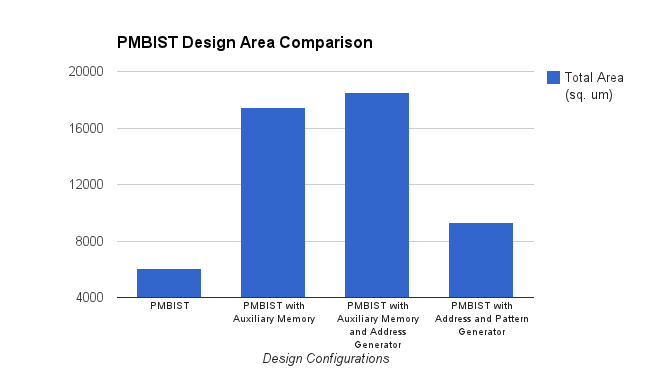
\includegraphics[width=\textwidth]{PMBIST_compare}
  \caption{Area Comparison of Different PMBIST Configurations}
  \label{fig:all_compare}
\end{figure}

Compared to the original base design, the design implemented in this report achieves a more robust address generation scheme while using less area than the orignal design thanks to the use of a pattern generator in place of an auxiliary memory.  As a final comparison the memory overheads for the various PMBIST designs discussed in this report are presented in Table \ref{tab:all_overhead}.  This table shows the percentage of the total memory IP block used by each of the PMBIST designs.  The design with combined address and pattern generation only increases the memory overhead by 1.8-9.6\% depending on memory size.  By comparison, the designs using auxiliary memory add an additional 6.3-26.5\% area overhead to the design.  

\begin{table}[h]
\caption{Area Overhead Added by PMBIST Designs}
\centering
\begin{tabular}{|c| c| c| c| c|}
\hline
Memory Size & Base Design & Base with Aux. Mem & AG with Aux. Mem & AG with PG  \\
\hline\hline
64x8   & 14706  & 29.2\% 54.3\% & 55.7\% & 38.8\% \\
128x8  & 15809  & 27.7\% 52.5\% & 54.0\% & 37.1\% \\
256x8  & 18258  & 24.9\% 48.9\% & 50.4\% & 33.8\% \\
512x8  & 23033  & 20.8\% 43.1\% & 44.6\% & 28.8\% \\
1024x8 & 32939  & 15.5\% 34.6\% & 36.0\% & 22.1\% \\
2048x8 & 52202  & 10.4\% 25.1\% & 26.2\% & 15.2\% \\
4096x8 & 91019  &  6.2\% 16.9\% & 16.9\% &  9.3\% \\
8192x8 & 171503 &  3.4\%  9.7\% &  9.7\% &  5.2\% \\ [0.5ex]
\hline
\end{tabular}
\label{tab:all_overhead}
\end{table}




